% generated from src/3 System design.md by tools/doc2tex.py; do not edit
\chapter{SYSTEM DESIGN AND IMPLEMENTATION}

\section{Architecture}

The system has two stages on one device. The detection runtime turns camera frames into skeletons on the Hailo-8, and the engagement analysis turns skeletons into a class-level share. Frames exist only in memory, and per-student states are never output by default.

\begin{figure}[htbp]
\centering
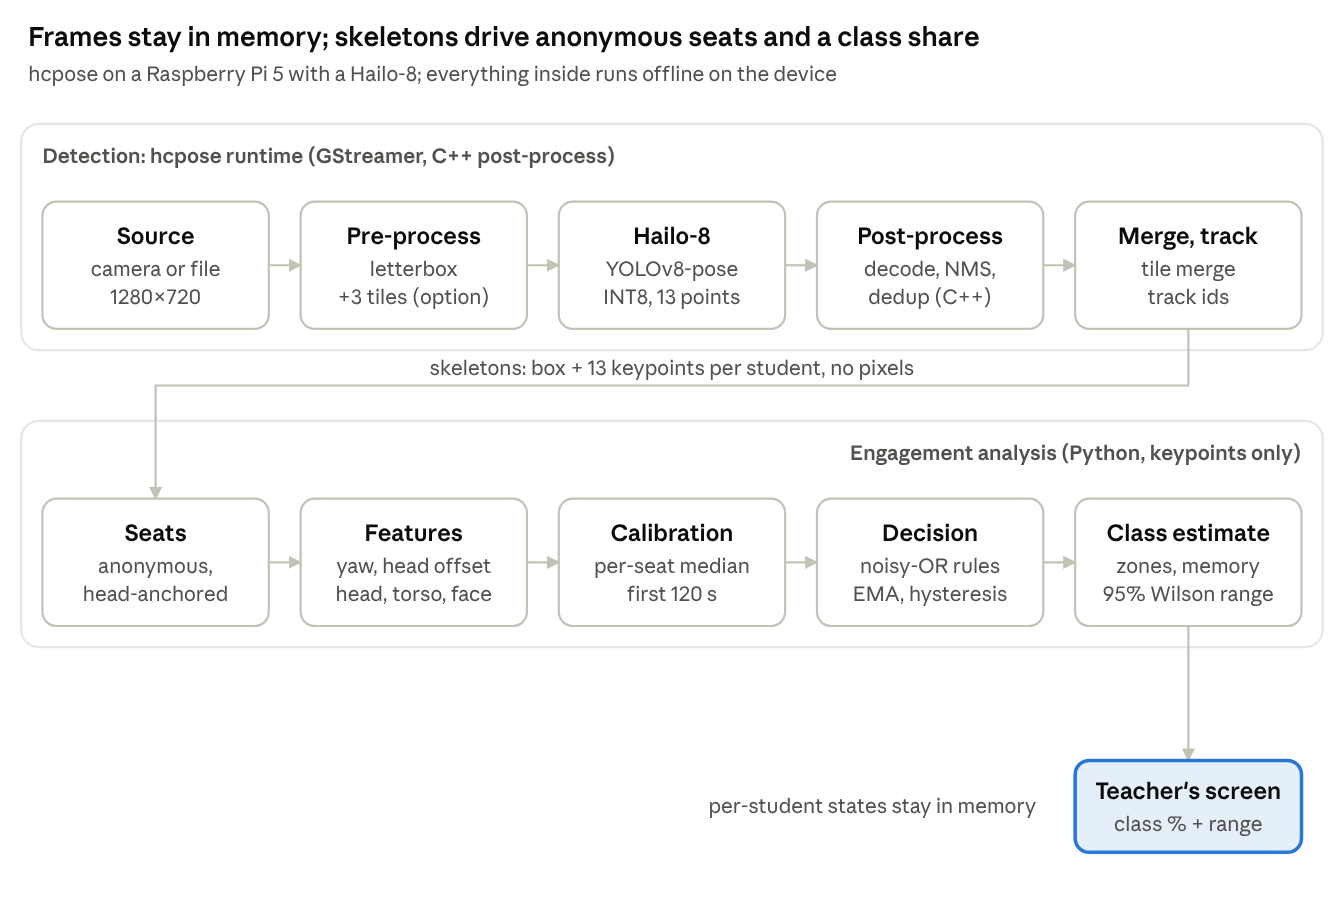
\includegraphics[width=1.0\textwidth]{figures/architecture.png}
\caption{Architecture of hcpose: frames stay in memory, and skeletons drive anonymous seats and a class-level share}\label{fig:architecture-of-hcpose-frames-stay-in-me}
\end{figure}

The skeleton file (\texttt{-\/-save-json}) and an annotated video (\texttt{-\/-output}) can be written at the hand-off between the two stages for development and evaluation. Both are off by default. The data-flow view used for the privacy analysis is in chapter 4.

\manualfigure{figures/manual/device}{The device}{The device: Raspberry Pi 5 with the Hailo-8 AI HAT+ (26 TOPS), active cooler and camera.}{fig:device}

\section{Pose models and compilation}

The pose models are YOLOv8-pose networks in three sizes, n, s and m, that predict one class (person) and 13 upper-body keypoints: COCO keypoints 0-12 \cite{b13}, from the nose to the hips. Classroom desks hide the legs, so the lower-body points carry no information. The models were trained on COCO with Ultralytics \cite{b14}, in the companion repository \texttt{hailo-custom-yolo-pose}, and kept fixed for this thesis.

\textbf{Training.} All three sizes start from Ultralytics' COCO-pretrained YOLOv8-pose weights. They were fine-tuned on COCO 2017 person keypoints: train2017 for training, val2017 for validation. The labels were converted with Ultralytics' \texttt{convert\_coco} and cut from 17 to 13 keypoints. The settings were the same for every size except the batch:

\begin{itemize}
\tightlist
\item
  100 epochs at 640×640; batch 16 for n and m, 32 for s; seed 0, deterministic mode, mixed precision.
\item
  \texttt{optimizer=auto}: Ultralytics chose the optimizer and learning rate itself, so the script's \texttt{lr0=0.01} and \texttt{momentum=0.937} were not used. The logged rates show a 3-epoch warm-up, then a linear fall to 1\% of the peak by epoch 100.
\item
  Loss weights and augmentation at Ultralytics defaults: HSV jitter, scale 0.5, translate 0.1, and horizontal flip at 0.5 with left and right keypoints swapped. Mosaic was on except in the last 10 epochs.
\end{itemize}

Training ran on the project's workstation (one NVIDIA RTX 3060) with Ultralytics' June 2026 release.

\begin{table}[htbp]\small
\caption{Training of the three pose models}\label{tab:training-of-the-three-pose-models}
\begin{tabularx}{\textwidth}{*{4}{>{\raggedright\arraybackslash}X}}
\toprule
\textbf{Model} & \textbf{Best epoch} & \textbf{Training time (h)} & \textbf{Box mAP50-95 (training log)} \\
\midrule
n & 100 & 43.1 & 0.527 \\
s & 99 & 42.4 & 0.584 \\
m & 96 & 89.9 & 0.619 \\
\bottomrule
\end{tabularx}
\end{table}

\textbf{Keypoint accuracy.} On COCO val2017 the trained models reach 0.470, 0.568 and 0.625 keypoint AP on their 13 points, 4-5 points below the stock 17-keypoint models on the same points. On the Hailo-8, INT8 costs n 5.3 points and m 6.8. The s HEF loses 30.8 points, so it is left out of every accuracy result.

\begin{table}[htbp]\small
\caption{Keypoint AP on COCO val2017, 13 upper-body keypoints, COCO tolerances}\label{tab:keypoint-ap-on-coco-val2017-13-upper-bod}
\begin{tabularx}{\textwidth}{*{5}{>{\raggedright\arraybackslash}X}}
\toprule
\textbf{Model} & \textbf{Stock 17-point model, on the 13 points} & \textbf{Trained 13-point model (.pt)} & \textbf{INT8 HEF on the Hailo-8} & \textbf{INT8 cost (AP points)} \\
\midrule
n & 0.523 & 0.470 & 0.417 & −5.3 \\
s & 0.613 & 0.568 & 0.260 & −30.8 \\
m & 0.665 & 0.625 & 0.557 & −6.8 \\
\bottomrule
\end{tabularx}
\end{table}

Keypoint AP (OKS 0.50:0.95) on the 5,000 val2017 images, scored with pycocotools \cite{b15} and COCO's per-keypoint tolerances. Every model gets the same 640×640 letterbox. As a check on the scoring, the stock models score 0.499, 0.594 and 0.645 on all 17 points, within 0.6 points of Ultralytics' published 50.4, 60.0 and 65.0.

\begin{itemize}
\tightlist
\item
  \textbf{Size.} m gains 0.14 AP over n on the Hailo-8 (0.557 against 0.417), for 4.7× the latency.
\item
  \textbf{Training on 13 points.} Most of the 4-5 point loss is in placing the face points precisely. With one loose tolerance for every point, the gap shrinks to 1.1-1.5 points.
\item
  \textbf{The s HEF.} It still finds people (AP50 0.683) but places keypoints poorly (AP75 0.127). On matched detections its median keypoint error is 4-9\% of the box size, against 2-3\% for the n and m HEFs, and every point is shifted the same way. The n model was compiled with the same script and is unaffected, so the fault is in this compile, not in the settings. The s model appears only in the speed results.
\item
  \textbf{Training-log scores.} The log's keypoint mAP50-95 (0.329, 0.376, 0.401) is far below the same models scored by pycocotools with the same uniform tolerance (0.579, 0.660, 0.706). The cause is people with no labelled keypoint among the 13. They make up 4,503 of the 10,777 people in the validation labels (41.8\%). pycocotools ignores them, but Ultralytics' validator counts them as targets it can never match. With those people removed, Ultralytics' own validator gives 0.555, 0.632 and 0.669, close to the pycocotools figures. The log therefore understates keypoint accuracy, and its keypoint scores are not used as results.
\end{itemize}

For the Hailo-8 each model is quantised to INT8 and compiled with the Hailo Dataflow Compiler into a HEF:

\begin{itemize}
\tightlist
\item
  \textbf{No on-chip NMS.} The nine raw head outputs are exported as end nodes: box distribution (DFL), class score and keypoints at strides 8, 16 and 32. Decoding and NMS run on the host, which keeps the HEF independent of the model's keypoint count.
\item
  \textbf{Sigmoid inside the HEF.} The class scores are passed through sigmoid inside the HEF. The runtime detects this per model, which fixed a double sigmoid in the code it replaced.
\end{itemize}

\begin{table}[htbp]\small
\caption{Throughput and latency of the INT8 HEFs on the Hailo-8 alone}\label{tab:throughput-and-latency-of-the-int8-hefs-}
\begin{tabularx}{\textwidth}{*{3}{>{\raggedright\arraybackslash}X}}
\toprule
\textbf{Model} & \textbf{Hailo-8 FPS} & \textbf{Hardware latency (ms)} \\
\midrule
n & 131.5 & 5.7 \\
s & 69.5 & 11.9 \\
m & 31.5 & 26.7 \\
\bottomrule
\end{tabularx}
\end{table}

\textbf{Quantisation.} The compiler (Hailo Dataflow Compiler 3.33.1, Model Zoo 2.18) calibrated the INT8 ranges on 1,024 random train2017 images resized to 640×640. The n and s models share one model script and m has its own. Both scripts keep three of the nine output layers at 16 bits; by their order these are the keypoint outputs. Both run Hailo's post-quantisation fine-tuning at learning rate 0.00015, and the n/s script also turns off pre-quantisation equalisation.

\section{Runtime: hcpose}

hcpose runs any YOLOv8-pose HEF on a Raspberry Pi 5. It reads the keypoint count, strides, tensor order, output data type and score activation from the HEF at start-up, so the same command runs the 13-keypoint models, the stock 17-keypoint model or others.

\textbf{Two engines, one result.}

\begin{itemize}
\tightlist
\item
  \textbf{GStreamer engine} (default, for live use): the camera or file source feeds \texttt{hailonet}. A C++ \texttt{hailofilter} decodes and post-processes the outputs, \texttt{hailotracker} assigns track ids, and \texttt{hailooverlay} draws.
\item
  \textbf{Python engine} (for images, debugging and evaluation): OpenCV and HailoRT with a NumPy decoder.
\item
  \textbf{Equivalence:} the two decoders produce identical detections, checked by the tests on recorded model outputs.
\end{itemize}

\textbf{Post-processing.}

\begin{itemize}
\tightlist
\item
  \textbf{Decoding:} DFL boxes and keypoints are decoded and mapped back through the letterbox.
\item
  \textbf{NMS:} candidates are sorted by score first. The inherited code skipped this, so overlaps were resolved by anchor order.
\item
  \textbf{Duplicate-skeleton removal:} after NMS, a box is dropped when it lies inside a stronger box and its skeleton matches: at least three common keypoints, closer on average than 0.1 × √(smaller box area). YOLO-pose often outputs a tight and a loose box for one student, and box NMS keeps both.
\end{itemize}

\textbf{Tiling for far rows.} With \texttt{-\/-tiles}, the model also runs on a row of overlapping, roughly square tiles over the top 60\% of the frame (three tiles at 1280×720).

\begin{itemize}
\tightlist
\item
  \textbf{In the GStreamer engine:} a custom crop function hands \texttt{hailocropper} the full frame plus the tiles. A second \texttt{hailofilter} after the aggregator merges the results.
\item
  \textbf{The merge:} tile detections are mapped to frame coordinates, those cut by an inner tile edge are dropped, and duplicates across passes are merged by IoU, or by containment plus agreeing keypoints.
\item
  \textbf{Checks:} the C++ merge equals the Python merge on 25 random scenes.
\item
  \textbf{Cost:} tiling multiplies inference by four.
\end{itemize}

\manualfigure{figures/manual/tiles}{The tiles}{Detections on the exam-hall clip without (left) and with (right) the three tiles over the far rows.}{fig:tiles}

\textbf{Outputs.}

\begin{itemize}
\tightlist
\item
  The annotated window, or headless operation.
\item
  Optionally an annotated video (\texttt{-\/-output}), for development only.
\item
  Optionally a JSON-lines skeleton file (\texttt{-\/-save-json}) with boxes and keypoints, no pixels.
\end{itemize}

\manualfigure{figures/manual/displays}{The two displays}{Left: development view with per-student states (green focused, red distracted, white calibrating). Right: the teacher's view, with the class share and its 95\% range only.}{fig:displays}

\section{Engagement analysis}

The analyzer turns each frame's skeletons into a focused, distracted or unknown state per student and a class-level share with a range. It works on keypoints alone and can replay a saved skeleton file (\texttt{hcpose\ analyze}) with any settings.

\textbf{Seats.} Students are tracked as anonymous seats, matched frame to frame by the top centre of their box (the head). The head stays put when a student leans or turns around, while the box centre jumps. A seat counts toward the class only while it is current and consistently seen.

\textbf{Features}, normalised by shoulder width:

\begin{itemize}
\tightlist
\item
  \textbf{Two head-turn measures.} Ear-based yaw: the nose between the ears. Head offset: the nose relative to the shoulder centre, which keeps working in profile.
\item
  \textbf{Head height} above the shoulder line.
\item
  \textbf{Torso ratio}, which shrinks when the body rotates.
\item
  \textbf{Face hidden} while the shoulders are visible.
\item
  \textbf{Hand raised}, and \textbf{hand at face}.
\end{itemize}

\textbf{Per-seat calibration.}

\begin{itemize}
\tightlist
\item
  Each seat learns its own attentive pose as the median of its first 120 s of usable observation. Before that, partial medians and the room's median are used.
\item
  The seat's yaw and head-offset baselines are kept within 0.3 and 0.15 of the room's, so a student who looks away during calibration does not learn ``turned'' as normal.
\item
  \texttt{-\/-camera-position} (left, centre, right) sets a prior for the room's attentive direction.
\end{itemize}

\textbf{Decision.} Each cue is a ramp from ``normal'' to ``clearly off'' relative to the seat's baseline. They combine with a noisy-OR, so weak cues such as head down (writing looks the same) only count together with another cue:

\begin{equation}
s = 1 - \prod_{c} \left(1 - w_c \, r_c\right)
\end{equation}

Here r\_c is cue c's ramp value and w\_c its weight. A raised hand overrides the score to 0. The default weights are: head turned 1.0, face hidden 0.9, head down 0.7, body turned 0.5, hand at face 0.4. The learned classifiers (trees, logistic regression, MLP) can replace the noisy-OR, but are off by default (chapter 4).

\textbf{Smoothing.} The score is smoothed with an exponential moving average (τ = 1 s) and switched with hysteresis:

\begin{itemize}
\tightlist
\item
  \textbf{to distracted:} above 0.6 for 2.5 s
\item
  \textbf{back to focused:} below 0.4 for 1.5 s
\item
  \textbf{unknown:} no usable keypoints for 2 s
\end{itemize}

This keeps brief glances from flipping a student.

\textbf{Class estimate.}

\begin{itemize}
\tightlist
\item
  Seats keep their last state for 15 s after they were last seen.
\item
  They are grouped into near, middle and far zones by image height, and each zone is weighted by its number of seats.
\item
  The class share comes with a 95\% Wilson interval \cite{b16} around the shown (smoothed) value. It is narrowed by the finite-population correction only when the real head count is given (\texttt{-\/-class-size}).
\item
  On screen: ``43\% distracted (20-65\%) \textbar{} 14 of \textasciitilde30 students''.
\end{itemize}

\section{Configuration, testing and reproducibility}

\textbf{Configuration.} Every threshold, weight and option is a setting in \texttt{configs/engagement.yaml} or a command-line flag:

\begin{itemize}
\tightlist
\item
  camera position
\item
  display mode (per-student, class, both or none)
\item
  class size
\item
  calibration file
\item
  classifier
\item
  tiling
\end{itemize}

A per-model sidecar YAML sets detection thresholds and keypoint names.

\textbf{Tests.} 44 automated tests cover:

\begin{itemize}
\tightlist
\item
  both decoders against recorded HEF outputs and Ultralytics' own decoding
\item
  the C++ letterbox mapping and tile merge against Python
\item
  the duplicate removal
\item
  the engagement logic on synthetic classes: calibration, glances, missing frames, seat counting, the interval, the head-offset measure
\item
  the staged-session scorer on a synthetic session with a known answer
\end{itemize}

\textbf{Reproducibility.} Results and the tools that made them are in the repository:

\begin{itemize}
\tightlist
\item
  skeleton files from the Pi
\item
  edge logs
\item
  the human labels
\item
  staged-session scripts
\item
  threshold sweeps
\end{itemize}

Every analysis can be rerun from the saved skeletons without the camera footage. The evaluated version is tagged \texttt{v1.0-thesis}.
